%% LaTeX-Beamer template for KIT design
%% by Erik Burger, Christian Hammer
%% title picture by Klaus Krogmann
%%
%% version 2.1
%%
%% mostly compatible to KIT corporate design v2.0
%% http://intranet.kit.edu/gestaltungsrichtlinien.php
%%
%% Problems, bugs and comments to
%% burger@kit.edu

\documentclass[19pt]{beamer}

%% SLIDE FORMAT

% use 'beamerthemekit' for standard 4:3 ratio
% for widescreen slides (16:9), use 'beamerthemekitwide'

\usepackage{templates/beamerthemekit}
\usepackage{wrapfig}

\usepackage[utf8]{inputenc}
\usepackage[T1]{fontenc}
\usepackage[ngerman]{babel}	% german hyphenation, quotes, etc
\usepackage{tikz}
\usepackage{hyperref}
\usepackage[export]{adjustbox}
% \usepackage[ngerman]{translator}

% \usepackage{templates/beamerthemekitwide}

%% TITLE PICTURE

% if a custom picture is to be used on the title page, copy it into the 'logos'
% directory, in the line below, replace 'mypicture' with the 
% filename (without extension) and uncomment the following line
% (picture proportions: 63 : 20 for standard, 169 : 40 for wide
% *.eps format if you use latex+dvips+ps2pdf, 
% *.jpg/*.png/*.pdf if you use pdflatex)
\titleimage{Gruppenarbeit_klein}

%% TITLE LOGO

% for a custom logo on the front page, copy your file into the 'logos'
% directory, insert the filename in the line below and uncomment it

\titlelogo{Logo_IOSB}

% (*.eps format if you use latex+dvips+ps2pdf,
% *.jpg/*.png/*.pdf if you use pdflatex)

%% TikZ INTEGRATION

% use these packages for PCM symbols and UML classes
% \usepackage{templates/tikzkit}
% \usepackage{templates/tikzuml}

% the presentation starts here

\title[PCC]{Privacy Crash Cam:\\ Implementierung}
\subtitle{App, Web-Interface und Web-Dienst}
\author{Giorgio G., Christoph H., David L.,  Josh R.,  Fabian W.}

\institute{Karlsruher Institut f\"ur Technologie, Fraunhofer Institut f\"ur Optronik, Systemtechnik und Bildauswertung}

% Bibliography

\usepackage[citestyle=authoryear,bibstyle=numeric,hyperref,backend=biber]{biblatex}
\addbibresource{templates/example.bib}
\bibhang1em

\begin{document}

% change the following line to "ngerman" for German style date and logos
\selectlanguage{ngerman}

%title page
\begin{frame}
	\titlepage
\end{frame}

%###############################################################################################

\section{Ausgangssituation}

\subsection{Vor der Implementierung}
\begin{frame}{Vor der Implementierung}
\begin{center}

\includegraphics[scale=0.2]{resources/start.jpg}
\end{center}
\end{frame}

\subsection{Ausgangssituation}
\begin{frame}{Ausgangssituation}
	\begin{itemize}
		\item Pflicht- (/Wunsch-) Kriterien Pflichtenheft
		\pause
		\item Entwurf
		\pause
		\item Einlesen und -arbeiten in Frameworks
		\pause
		\item Auseinandersetzung mit den Entwicklungsumgebungen
		\pause
		\item Schreiben von Demos
	\end{itemize}
\end{frame}

\section{Implementierung}

\subsection{Fakten schaffen}
\begin{frame}{Fakten schaffen}
\begin{center}
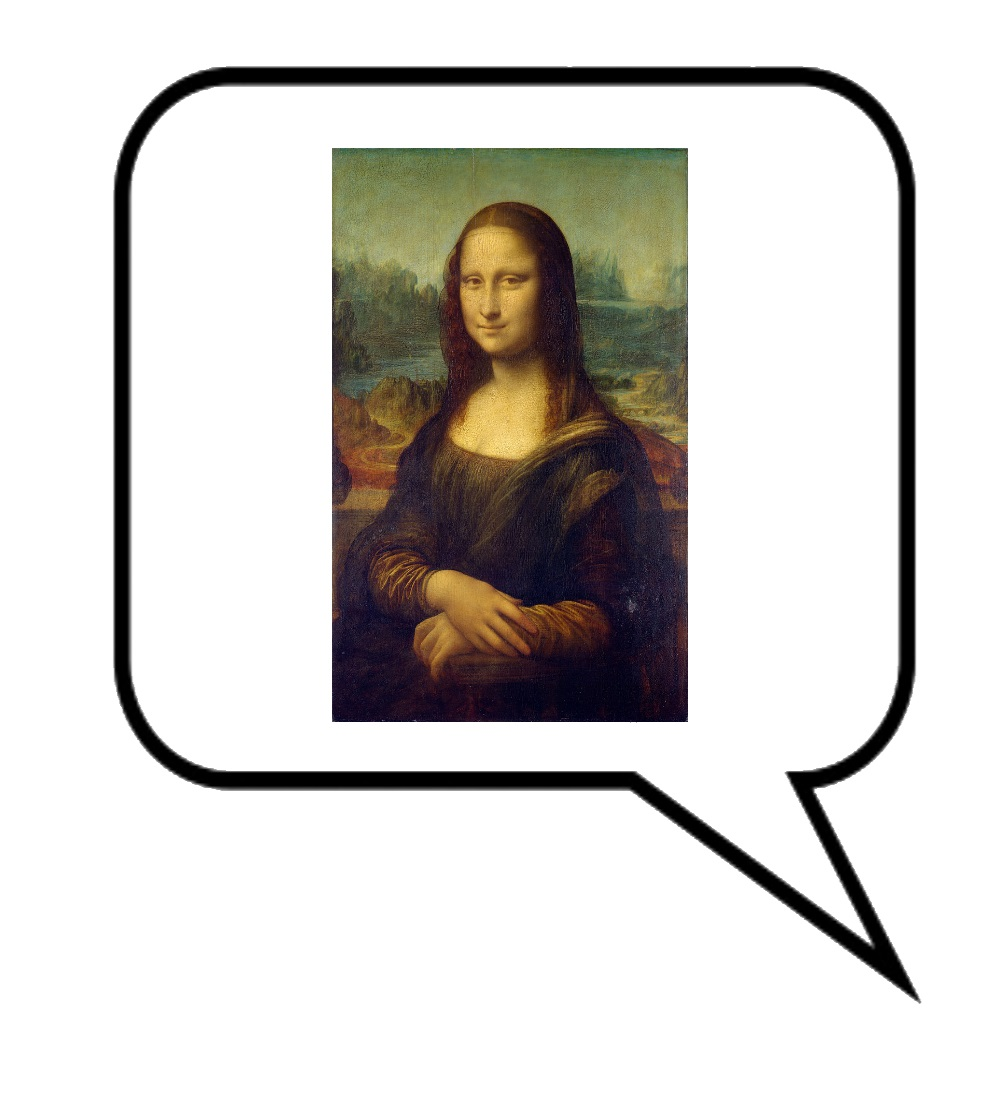
\includegraphics[scale=0.2]{resources/start2.jpg}
\end{center}
\end{frame}

\subsection{Aufgaben}
\begin{frame}{Aufgaben}
	\begin{itemize}
		\item Planung
		\pause
		\begin{itemize}
			\item Aufgaben sammeln (JIRA)
			\pause
			\item Leitfaden bestimmen
			\pause
			\item Implementierungsplan
			\pause
			\item auf Styling (Layout, Javadoc, Formatter) einigen
			\pause
		\end{itemize}
		\item Durchführung
		\pause
		\begin{itemize}
			\item Projekte aufsetzen (IntelliJ/Android Studio)
			\pause
			\item Implementierung
			\pause
			\item Dokumentation
			\pause
			\item Testen
			\pause
			\item ausführbare Instanzen bauen
		\end{itemize}
	\end{itemize}
\end{frame}

\subsection{Aufgaben sammeln}

\begin{frame}{Aufgaben sammeln}
	\begin{center}
		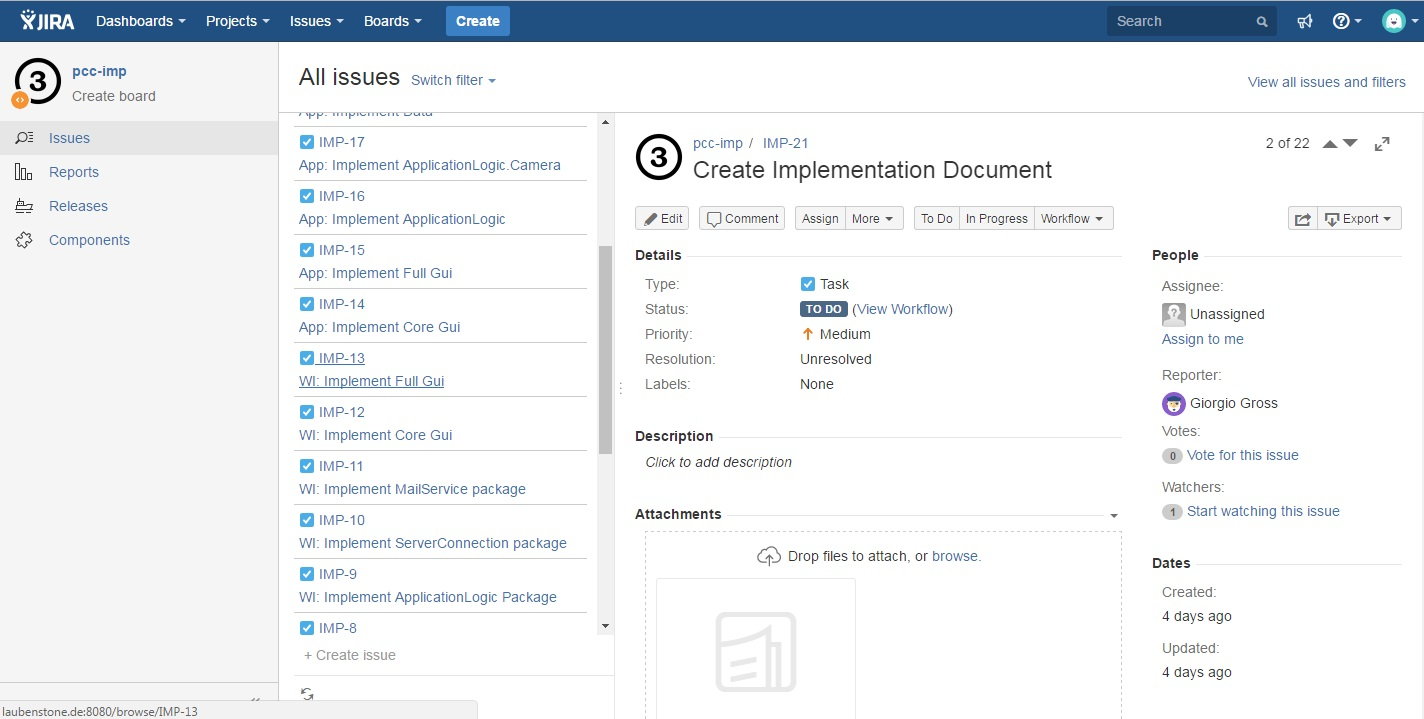
\includegraphics[scale=0.3]{resources/Jira.jpg}
	\end{center}
\end{frame}

\subsection{Implementierungsplan}

\begin{frame}{Implementierungsplan}
	\begin{center}
		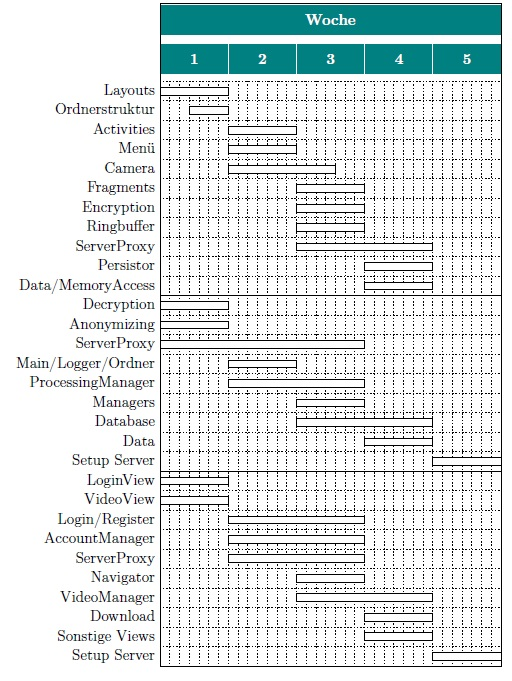
\includegraphics[scale=0.4]{resources/ImpPlanPre.jpg}
	\end{center}
\end{frame}

\subsection{Projekte aufsetzen}

\begin{frame}{Projekte aufsetzen}
\begin{center}
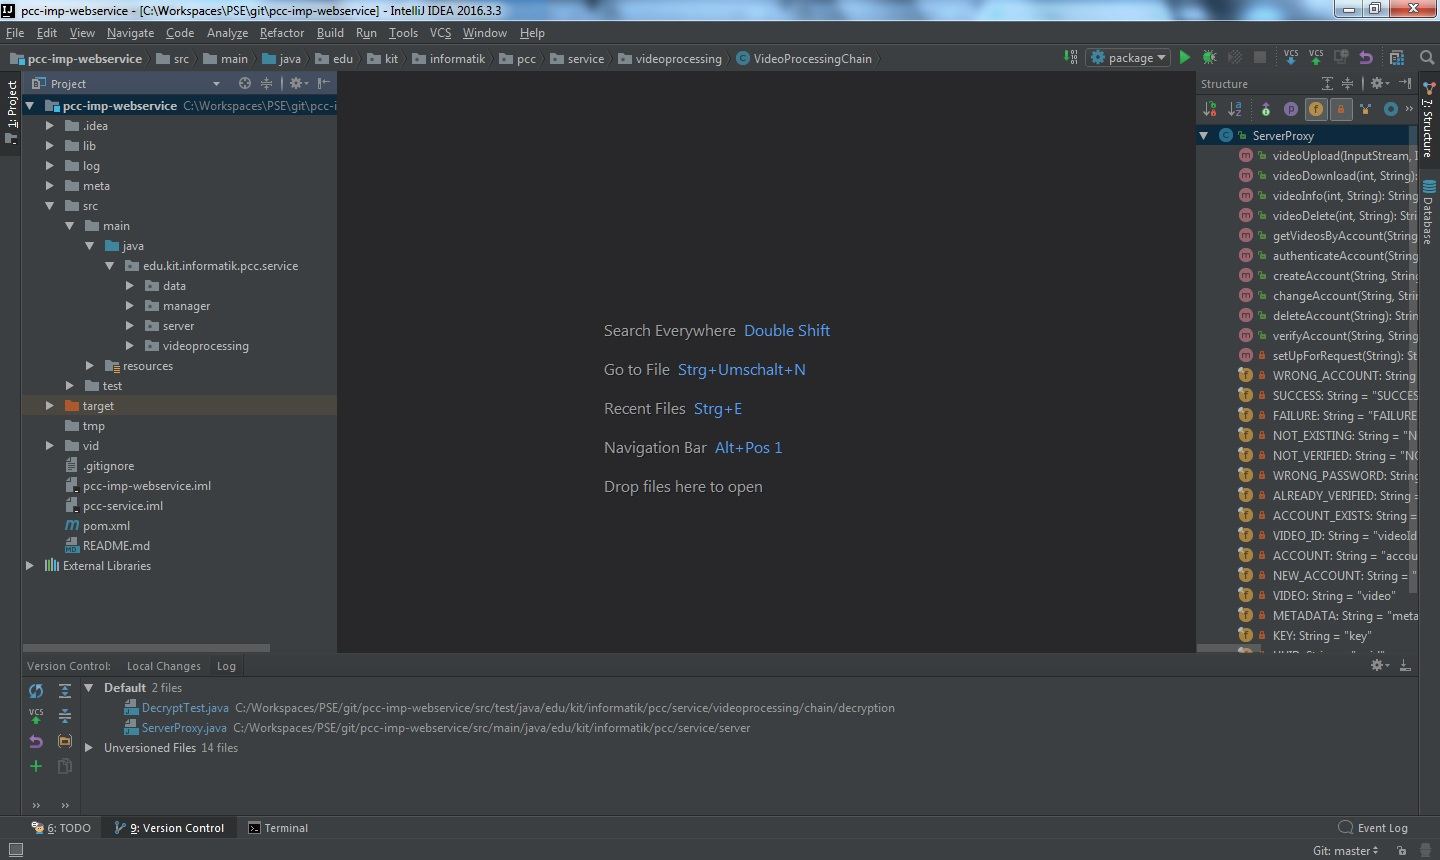
\includegraphics[scale=0.3]{resources/Projekt.jpg}
\end{center}
\end{frame}

\section{Probleme}

\subsection{Intro}
\begin{frame}{Probleme}
	Wir sind leider
	\begin{center}
        \begin{figure}
				
\includegraphics[scale=0.35]{resources/Wahrsager.jpg}
				
\includegraphics[scale=0.35]{resources/zauberer.jpg}
				
\includegraphics[scale=0.7]{resources/Hacker.jpg}
		\end{figure}
	\end{center}
	$\rightarrow$ Es sind Probleme aufgetreten
\end{frame}

\subsection{Probleme und Folgen}
\begin{frame}{Probleme (1): Ringbuffer}
	\begin{itemize}
		\item Probleme mit Asynchronität des MediaRecorders
		\pause
		\item Warten auf Fertigstellung der Videoschnipsel vor weiterer Bearbeitung
		\pause
		\item[$\rightarrow$] 1. Versuch: FileObserver auf Videoschnipseln
		\pause
		\item Nicht alle Events wurden gefangen
		\pause
		\item[$\rightarrow$] Lösung: FileObserver auf Ordner
	\end{itemize}
\end{frame}

\begin{frame}{Probleme (2): Maven Service}
	\begin{itemize}
		\item Probleme mit OpenCv, da OpenCv keine Maven-Schnittstelle besitzt.
		\pause
		\item Zudem benötigt OpenCv native libraries.
		\pause
		\item[$\rightarrow$] Lösung Java: Verwaltung über maven-dependency-plugin
		\pause
		\item[$\rightarrow$] Lösung natives: manuelle Installation
	\end{itemize}
\end{frame}

\begin{frame}{Probleme (3): Vaadin}
	\begin{itemize}
		\item Probleme mit der Vor- bzw. Zurückfunktion der Browser.
		\pause
		\item Probleme mit dem FileDownloader
		\pause
		\item Probleme mit Layouts
		\pause
		\item Probleme mit Vaadin
		\pause
		\item[$\rightarrow$] Das Interface verbietet Navigation zwischen Login-View und anderen Views durch Browserfunktionen.
		\pause
		\item[$\rightarrow$] File Proxy, der das Video bei Anfragen lädt
		\pause
		\item[$\rightarrow$] In Zukunft kein Vaadin für kleine Projekte
	\end{itemize}
\end{frame}

\begin{frame}{Probleme (3): Ergänzungen/Änderungen}
	\begin{itemize}
		\item Bei der Implementierung sind Lücken/Ungenauigkeiten im Entwurf aufgefallen. Zudem entstanden Ideen, wie man Dinge verbessern kann.
		\pause
		\item[$\rightarrow$] es wurden einige Ergänzungen/ Änderungen nötig
		\pause
		\begin{itemize}
			\item neue Methoden, z.B. cleanUp() in VideoProcessingChain
			\pause
			\item neue Konstanten/Enumerations für Rückgabewerte oder Parameter, z.B. VideoProcessingChain.Chain, Konstanten im ServerProxy
			\item neue/andere Parameter, z.B. im Encryption-Modul der App
			\pause
			\item Ergänzungen in der Datenbank, z.B. Salt für das Hashen
			\pause
			\item Umbenennungen, z.B. Ringbuffer $\rightarrow$ VideoRingBuffer
		\end{itemize}
	\end{itemize}
\end{frame}

\begin{frame}{Erfolge}
	\begin{itemize}
		\item Einige Dinge liefen sogar schneller als ursprünglich geplant
		\pause
		\begin{itemize}
			\item App-Layout
			\pause
			\item App-Camera
			\pause
			\item Web-Service VideoProcessing-Modul
			\pause
			\item Web-Service Server setup
			\pause
			\item Web-Interface Video download
		\end{itemize}
	\end{itemize}
	
\includegraphics[scale=0.2,right]{resources/Daumen.jpg}
\end{frame}

\section{Ergebnis}

\subsection{Tatsächlicher Implementierungsplan}
\begin{frame}{Tatsächlicher Implementierungsplan}
\begin{center}
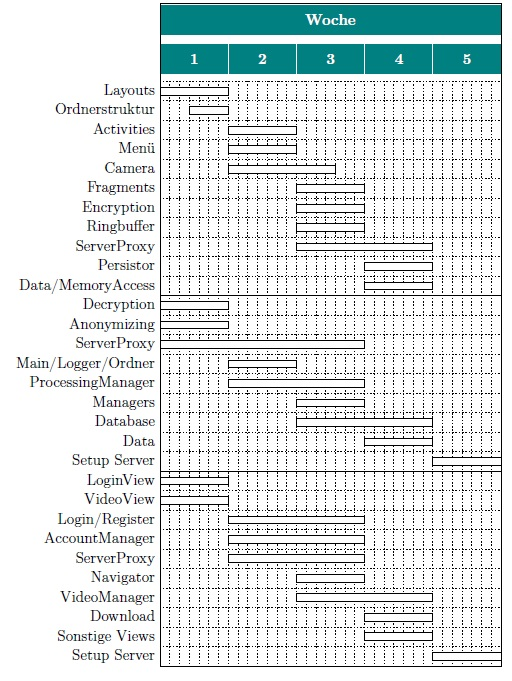
\includegraphics[scale=0.4]{resources/ImpPlanPre.jpg}
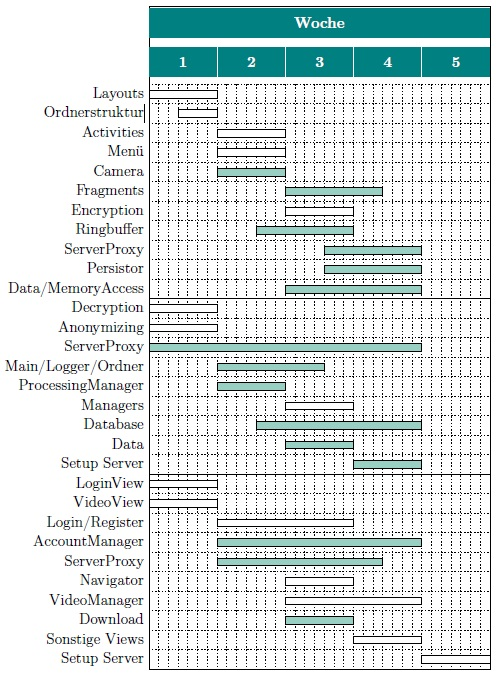
\includegraphics[scale=0.4]{resources/ImpPlanPost.jpg}
\end{center}
\end{frame}

\subsection{Code}
\begin{frame}{Code}
\begin{center}
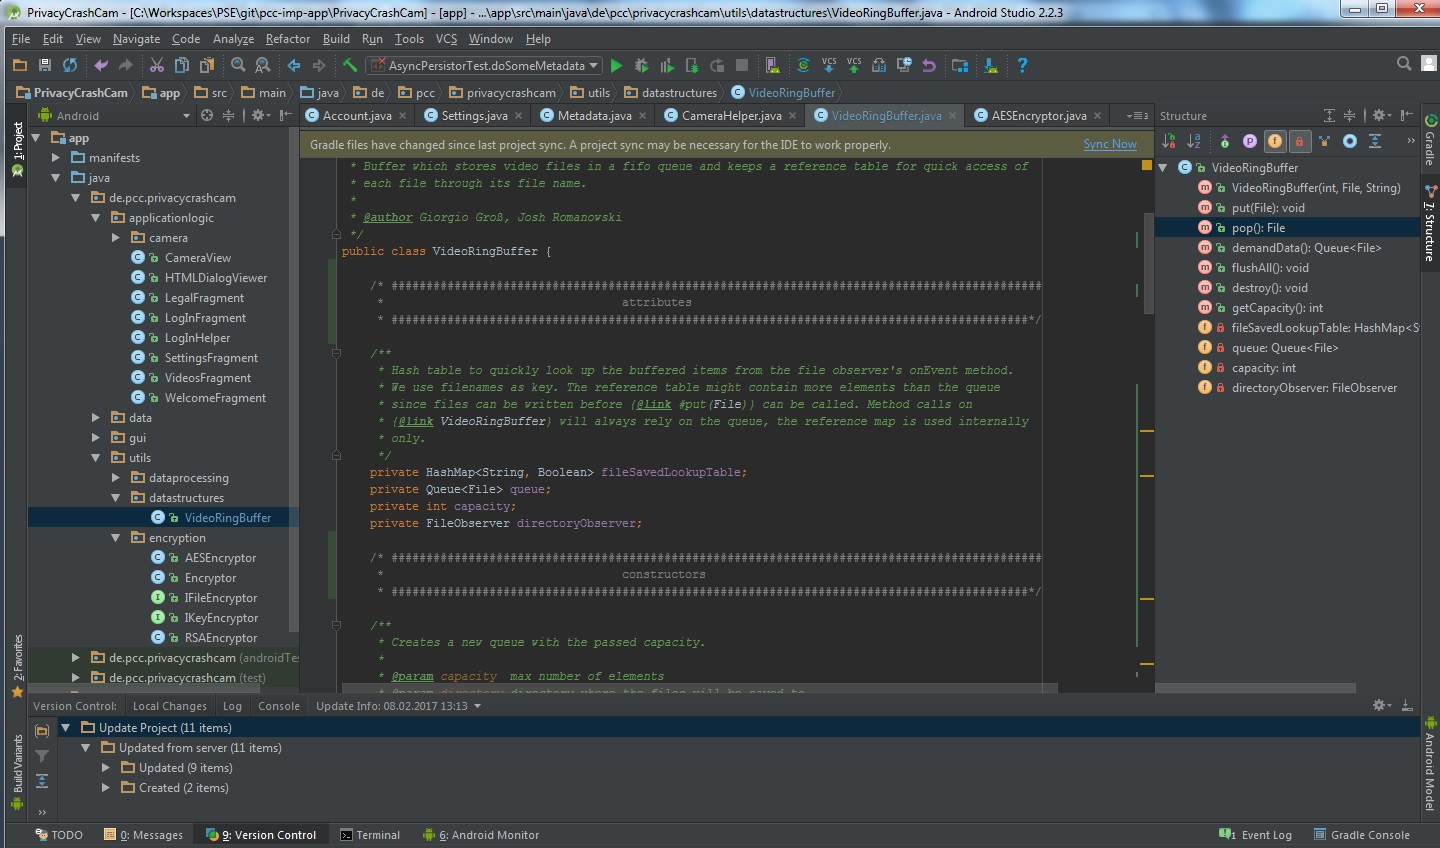
\includegraphics[scale=0.3]{resources/Code.jpg}
\end{center}
\end{frame}

\subsection{Oberfläche}
\begin{frame}{Oberfläche (1)}
\begin{center}
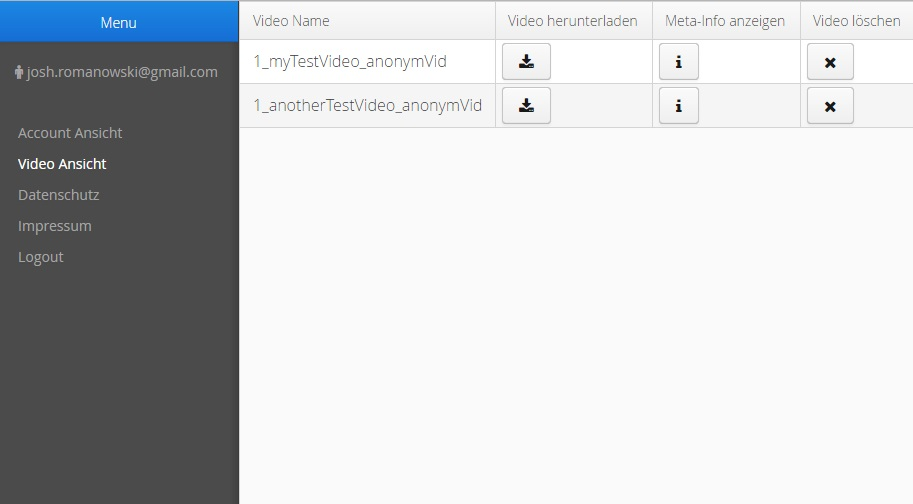
\includegraphics[scale=0.4]{resources/ServiceDemo.jpg}
\end{center}
\end{frame}

\begin{frame}{Oberfläche (2)}
\begin{center}
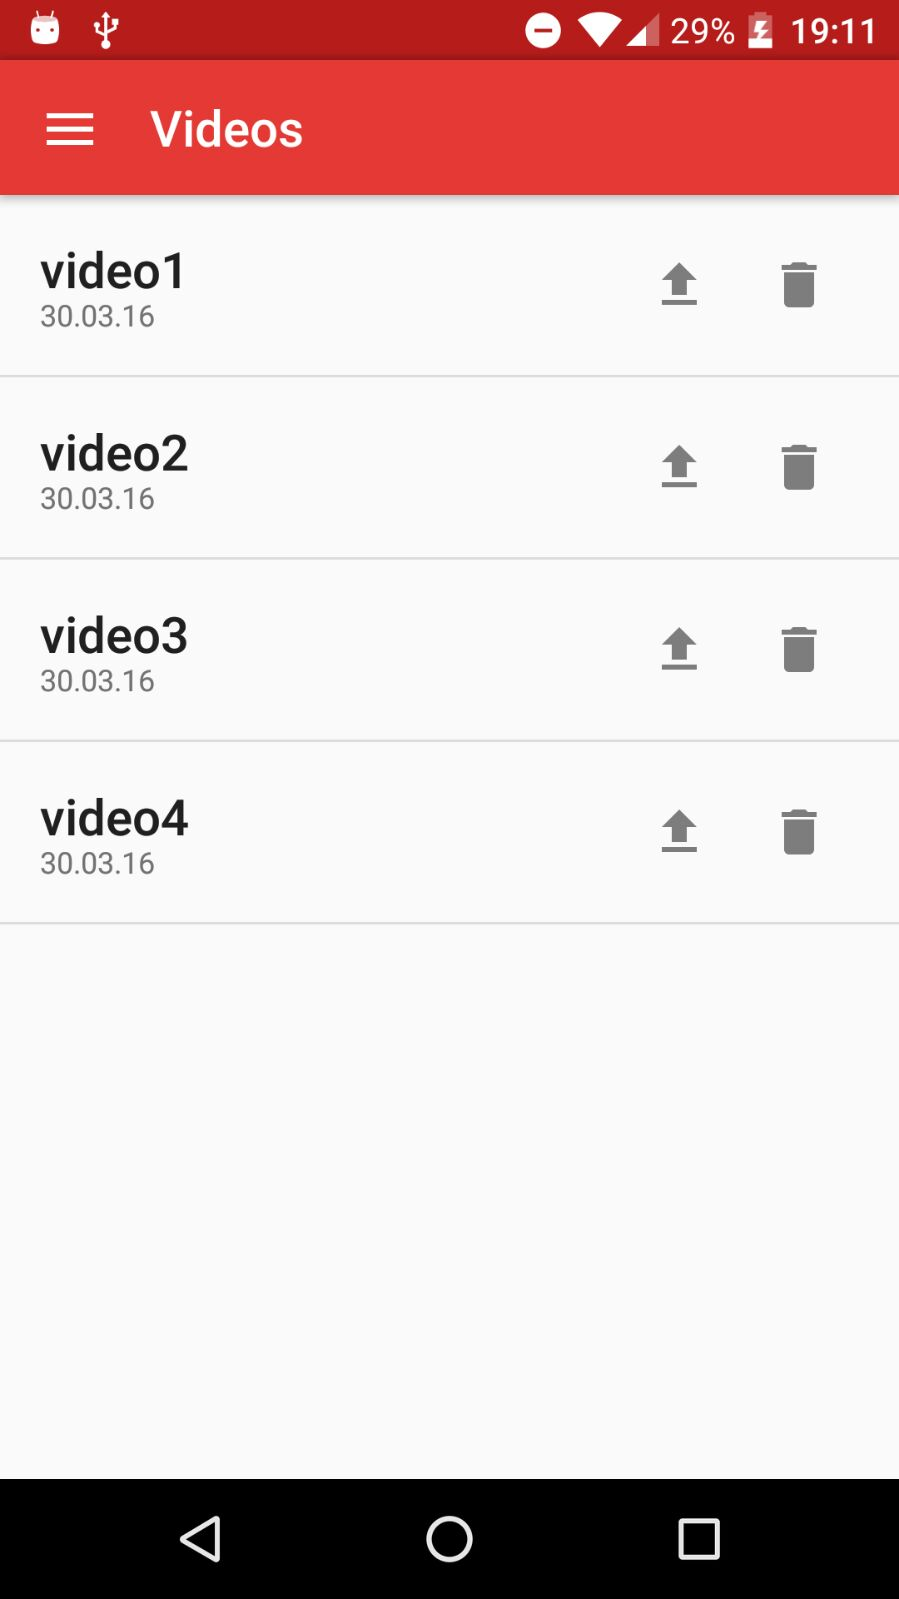
\includegraphics[scale=0.1]{resources/AppDemo.jpg}
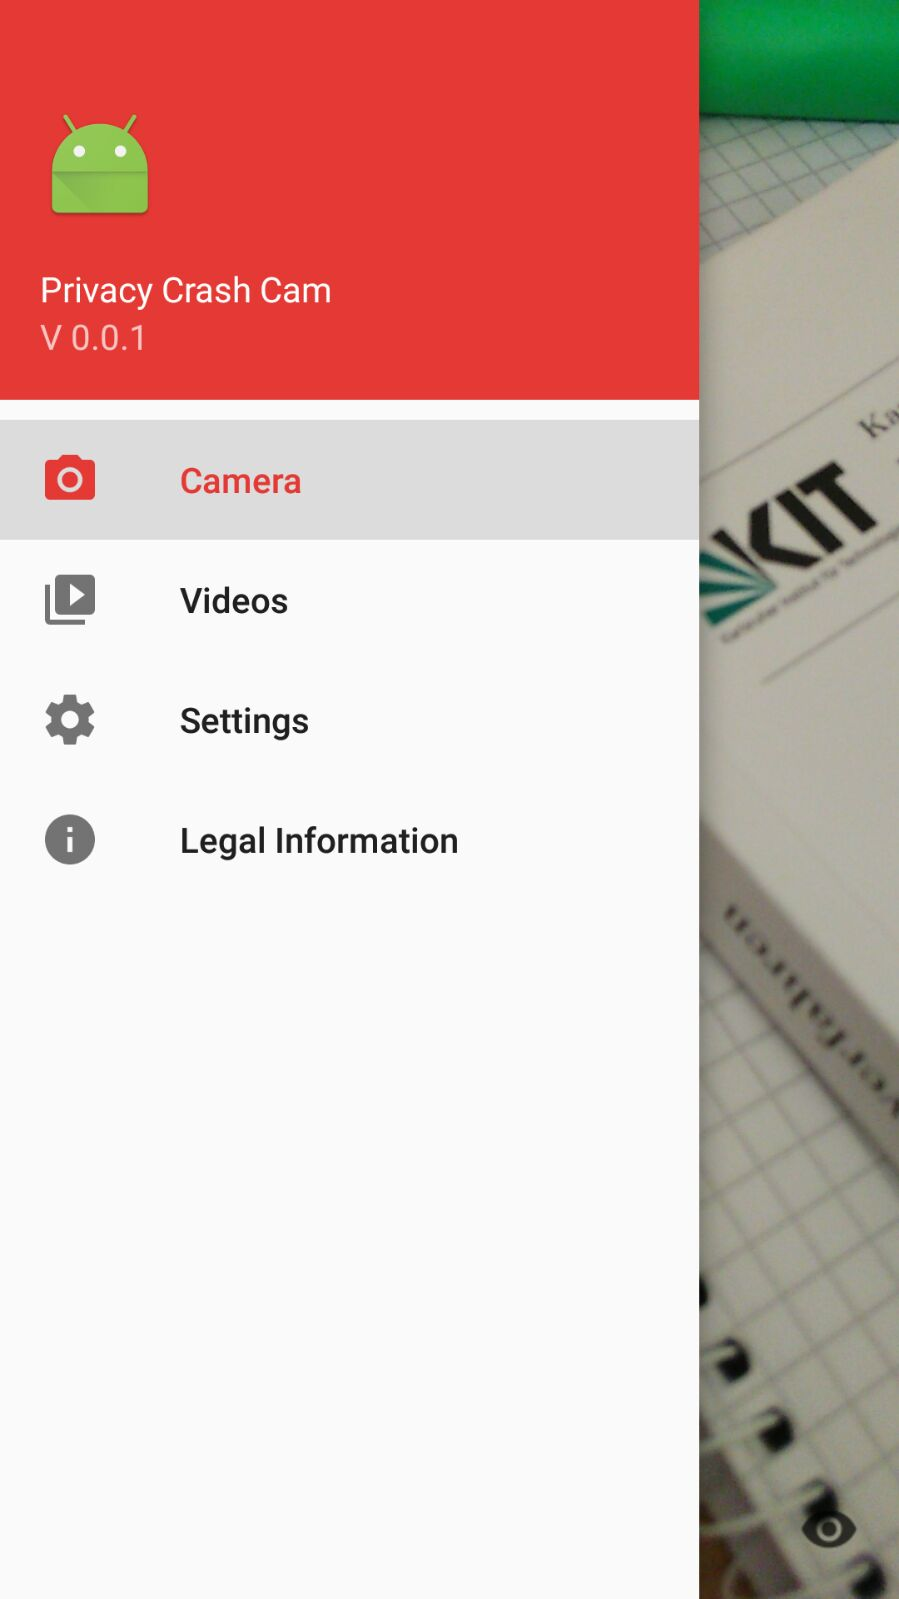
\includegraphics[scale=0.1]{resources/AppDemo2.jpg}
\end{center}
\end{frame}

\subsection{Final}
\begin{frame}{Endergebnis}
\begin{center}
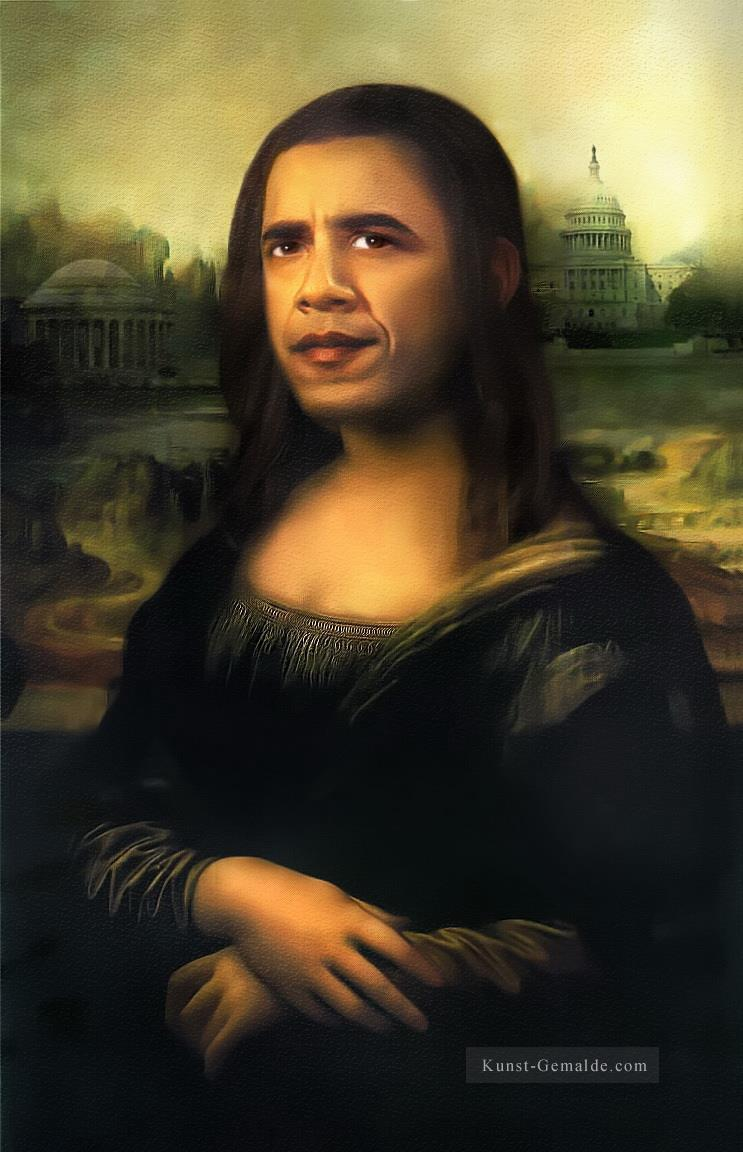
\includegraphics[scale=0.2]{resources/final.jpg}
\end{center}
\end{frame}

\section{Organisation}

\subsection{Aufgabenverteilung}
\begin{frame}{Aufgabenverteilung}
  \begin{columns}[T]
    \begin{column}{.5\textwidth}
    		\begin{itemize}
    	\item Christoph H.
			\begin{itemize}
				\item Web-Interface
				\item Präsentation
			\end{itemize}
		\item David L.
			\begin{itemize}
				\item Web-Dienst
				\item App (Data)
			\end{itemize}
		\item Fabian W.
			\begin{itemize}
				\item Web-Dienst
				\item ServerProxy App/Interface
			\end{itemize}
    		\end{itemize}
    \end{column}
    \begin{column}{.5\textwidth}
    \begin{itemize}
		\item Giorgio G.
			\begin{itemize}
				\item App
			\end{itemize}
		\item Josh R.
			\begin{itemize}
				\item Web-Dienst
				\item App (Utility)
			\end{itemize}
	\end{itemize}
    \end{column}
  \end{columns}
\end{frame}

\subsection{Github}
\begin{frame}{Github (Stand 10.2.17)}
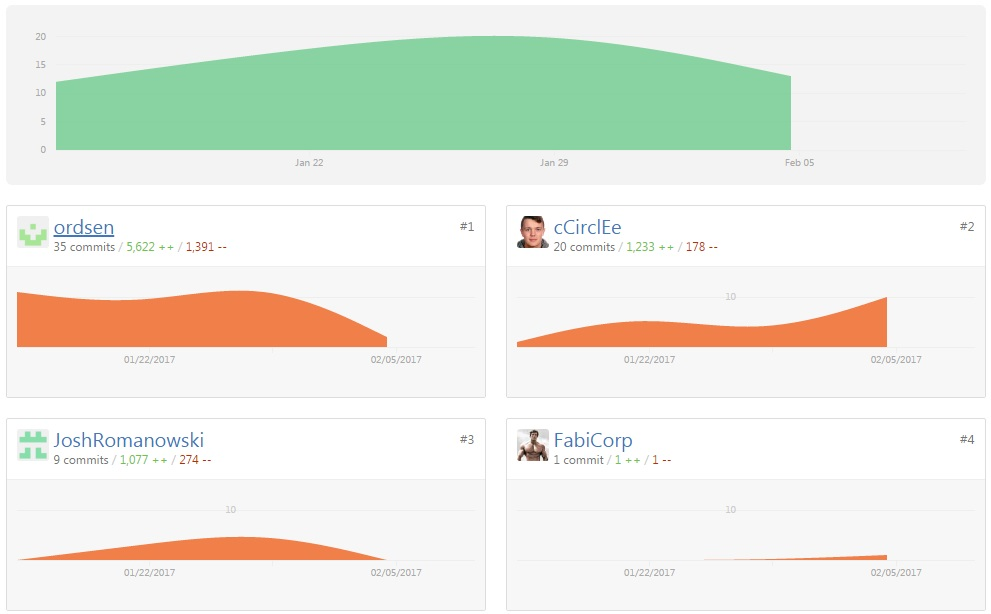
\includegraphics[scale=0.2]{resources/GithubApp.jpg}
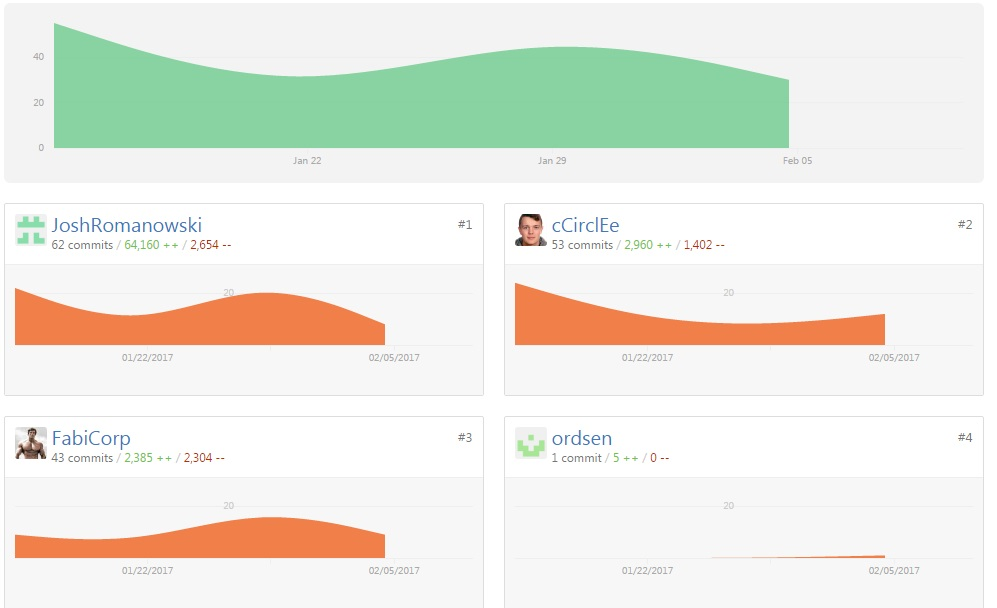
\includegraphics[scale=0.2]{resources/GithubService.jpg} \\
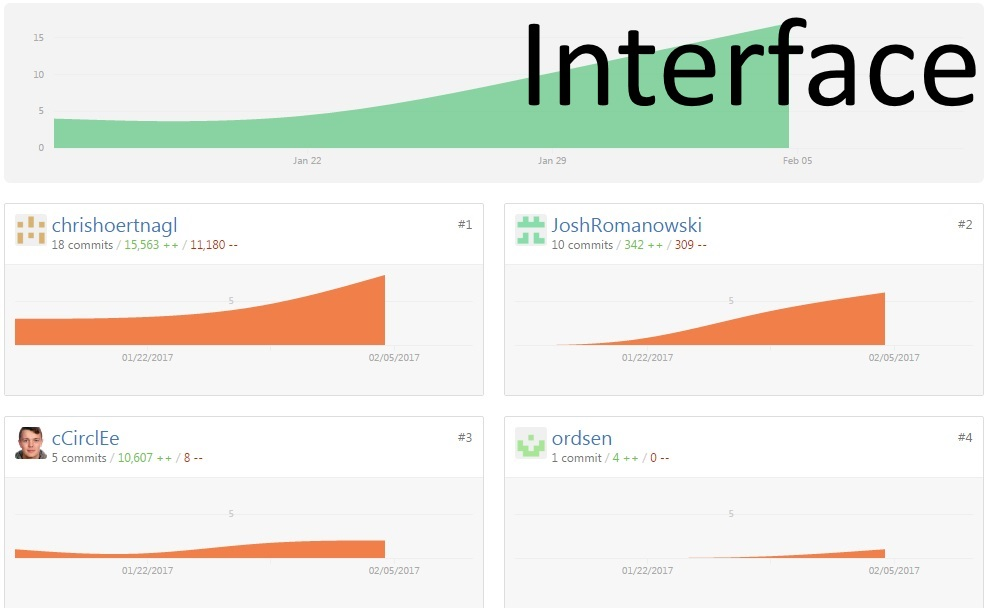
\includegraphics[scale=0.2]{resources/GithubInterface.jpg}
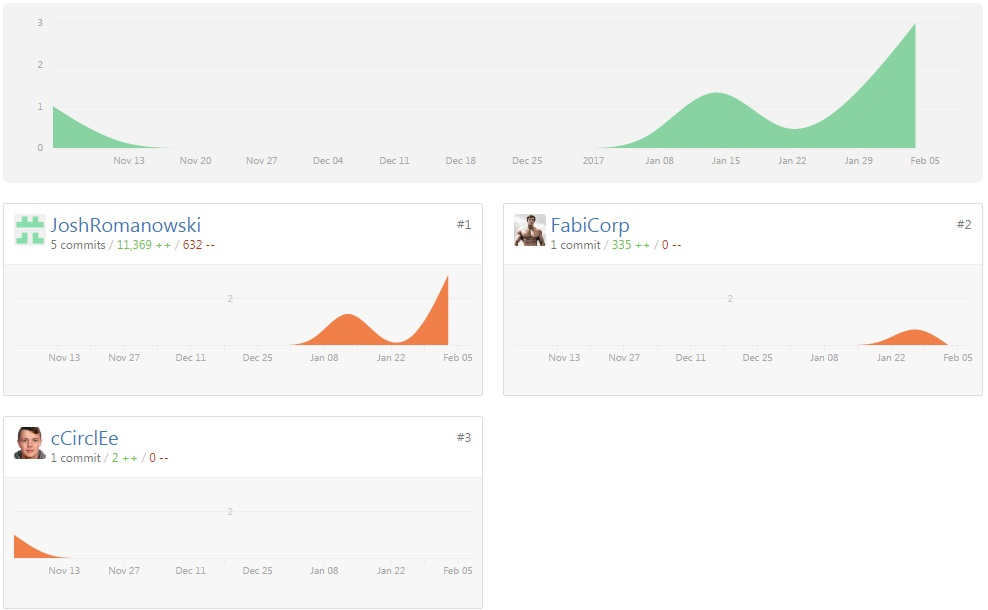
\includegraphics[scale=0.2]{resources/GithubImp.jpg}
\end{frame}

\section{Gruppenarbeit}
\begin{frame}{Gruppenarbeit}
	\begin{figure}
		\begin{center}
			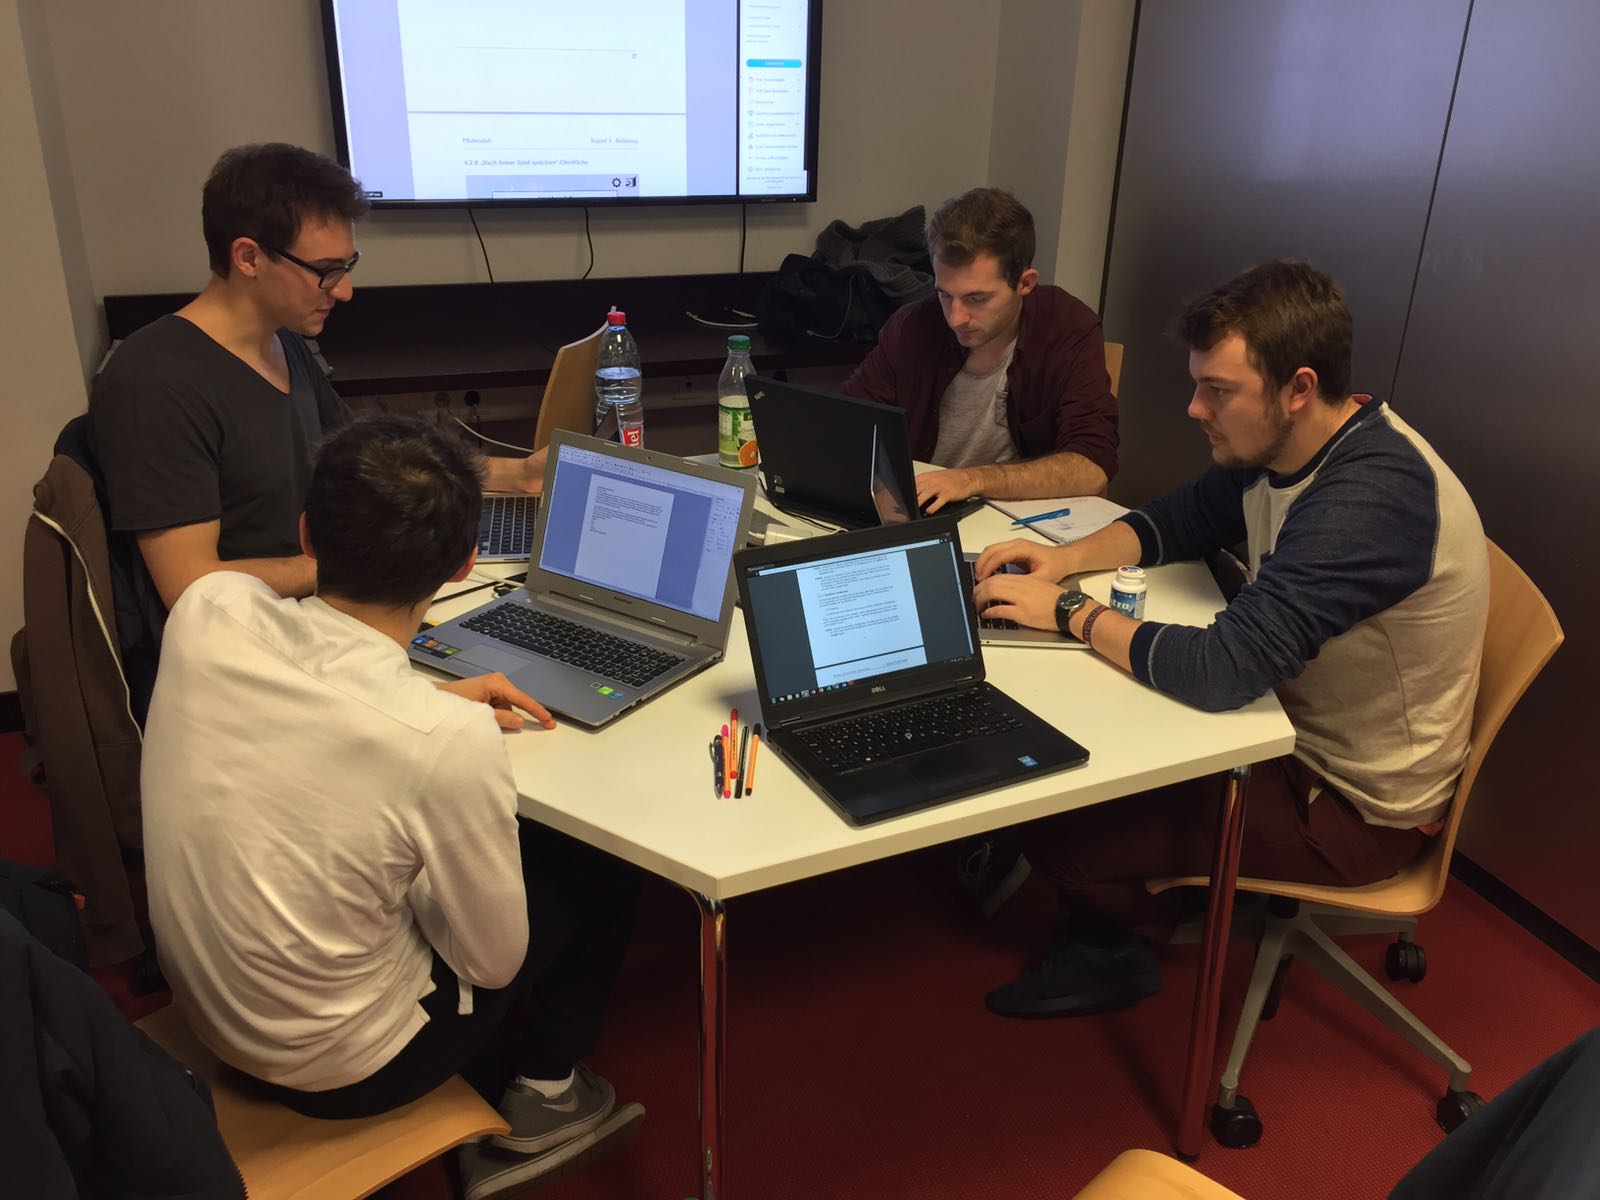
\includegraphics[scale=0.16]{resources/Gruppenarbeit} 
		\end{center}
	\end{figure}	 
\end{frame}

\section{Quellen}
\begin{frame}{Quellen}
	\begin{itemize}
		\item \url{http://de.clipartlogo.com/free/rain-cloud-cartoon.html}
		\item \url{https://www.spreadshirt.de/sprechblase+-+comic+t-shirts}
		\item \url{https://de.wikipedia.org/wiki/Mona_Lisa}
		\item \url{https://nebadonia.wordpress.com/2015/09/17/erkenne-die-matrix-und-wie-komme-ich-da-raus/}
		\item \url{http://ausmalbilder.kim/category/malvorlagen/zauberer/}
		\item \url{https://www.gratis-malvorlagen.de/phantasie/wahrsagerin-3/}
		\item \url{https://www.spreadshirt.de/daumen+geschenke}
	\end{itemize}
\end{frame}

\end{document}
